\documentclass[12pt]{article}%
\usepackage{amsfonts}
\usepackage{fancyhdr}
\usepackage{comment}
\usepackage[a4paper, top=2.5cm, bottom=2.5cm, left=2.2cm, right=2.2cm]%
{geometry}
\usepackage{times}
\usepackage{amsmath}
\usepackage{changepage}
\usepackage{amssymb}
\usepackage{ifthen}
\usepackage{graphicx}%
\setcounter{MaxMatrixCols}{30}
\newtheorem{theorem}{Theorem}
\newtheorem{acknowledgement}[theorem]{Acknowledgement}
\newtheorem{algorithm}[theorem]{Algorithm}
\newtheorem{axiom}{Axiom}
\newtheorem{case}[theorem]{Case}
\newtheorem{claim}[theorem]{Claim}
\newtheorem{conclusion}[theorem]{Conclusion}
\newtheorem{condition}[theorem]{Condition}
\newtheorem{conjecture}[theorem]{Conjecture}
\newtheorem{corollary}[theorem]{Corollary}
\newtheorem{criterion}[theorem]{Criterion}
\newtheorem{definition}[theorem]{Definition}
\newtheorem{example}[theorem]{Example}
\newtheorem{exercise}[theorem]{Exercise}
\newtheorem{lemma}[theorem]{Lemma}
\newtheorem{notation}[theorem]{Notation}
\newtheorem{problem}[theorem]{Problem}
\newtheorem{proposition}[theorem]{Proposition}
\newtheorem{remark}[theorem]{Remark}
\newtheorem{solution}[theorem]{Solution}
\newtheorem{summary}[theorem]{Summary}
\newenvironment{proof}[1][Proof]{\textbf{#1.} }{\ \rule{0.5em}{0.5em}}

\newcommand{\Q}{\mathbb{Q}}
\newcommand{\R}{\mathbb{R}}
\newcommand{\C}{\mathbb{C}}
\newcommand{\Z}{\mathbb{Z}}

\begin{document}

\title{Assignment 5}
\author{Changwoon Choi \\ 2020-20206}
\date{\today}
\maketitle

\section{Logistic Regression}
Suppose you train a logistic regression classifier and your hypothesis function is $H_\theta (x) = g(\theta_0 + \theta_1 x_1 + \theta_2 x_2 ).$ Where $g$ is logistic function and $\theta_0 , \theta_1 ,$ and $\theta_2$ are 6, 0, and -1, respectively. Draw the decision boundaries for classification and indicate where the positive prediction is.
\\

Ans) \\
\begin{figure}[h]
	\centering
	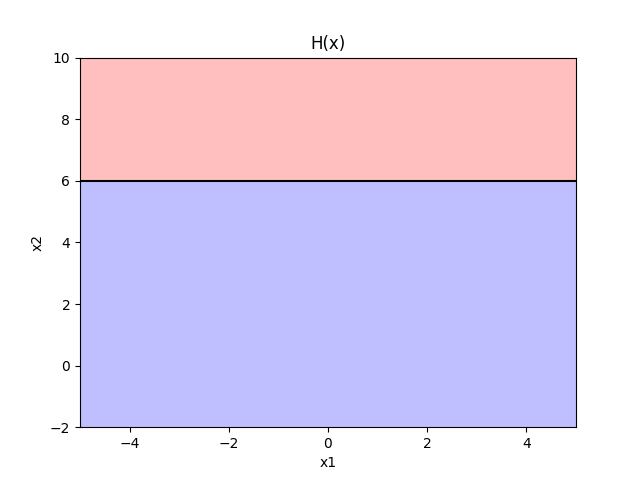
\includegraphics[scale=0.5]{problem_1}
	\caption{graph of $H_\theta (x)$, black line indicates the decision boundaries and the red region stands for the negative prediction and vice versa.}
\end{figure}


\section{Logistic function}
The logistic function is defined as $g(z) = {1 \over 1 + e^{-z}}$. It is known that the logistic function is easy to differentiate because it has a simple derivative $ {\partial \over \partial z}g(z) = g(z)(1 - g(z)).$ Derive this equation.\\

Ans) 
\begin{equation}
	\begin{aligned}
		{\partial \over {\partial z}} g(z) & = {\partial \over {\partial z}} {1 \over {1 + e^{-z}}}\\
		& = {\partial \over {\partial z}} {e^z \over {e^z + 1}} \\
		& = {{e^z (e^z + 1) - e^z e^z} \over {(1 +e^z )^2}} \\
		& = {e^z \over {(1 +e^z )^2}} \\
		& = {e^z \over {1 +e^z }} {1 \over {1 +e^z }} \\
		& = {1 \over {1 +e^{-z} }} {e^{-z} \over {1 +e^{-z} }} \\
		& = g(z) (1 - g(z))
	\end{aligned}
\end{equation}

\section{Gradient descent for logistic regression}
Using the equation above, derive the gradient descent algorithm for logistic regression.\\

Ans)


\section{Cost function for logistic regression}
Derive the cost function $J(\theta)$ from the perspective of the maximum (log) likelihood; i.e. by maximizing the joint probability of $m$ training samples being correctly classified. (Hint: the probability of $y=1$ or $0$, given $x$, parameterized by $\theta$ can be written more compactly as $P(y | x; \theta) = (h_\theta (x))^y (1 - h_\theta (x))^{1-y} )$)\\

Ans)\\
Assume ($\mathbf{x_1}$, $y_1$), ($\mathbf{x_2}$, $y_2$)), $...$ , ($\mathbf{x_N}$, $y_N$) are independently generated (iid assumption).\\
probability of getting all $y_n$'s from corresponding $\mathbf{x_n}$'s:
\begin{equation}
	P(y_1 | \mathbf{x_1})P(y_2 | \mathbf{x_2}) ... P(y_N | \mathbf{x_N}) = \prod_{n=1}^{N} {P(y_n | \mathbf{x_n})}
\end{equation}
From the perspective of the maximum likelihood, selects the hypothesis $h$ that maximizes this probability.\\
We can equivalently minimize a more convenient quantity: 
\begin{equation}
	- {1 \over N} \ln (\prod_{n=1}^{N} {P(y_n | \mathbf{x_n})}) = {1 \over N} \ln \sum_{n=1}^{N} {1 \over P(y_n | \mathbf{x_n})}
\end{equation}
( $\because - {1 \over N} \ln(x)$ is a monotonically decreasing function.)\\
The likelihood would be:
\begin{equation}
	P(y | \mathbf{x}) = 
	\begin{cases}
		g(\mathbf{\theta}^T\mathbf{x}) & \text{for $y = +1$}\\
		1 - g(\mathbf{\theta^T}\mathbf{x}) & \text{for $y = -1$}\\
	\end{cases}
\end{equation}

eq (4) can be write as,
\begin{equation}
	P(y | \mathbf{x})=  g(y \theta^T \mathbf{x})
\end{equation}

\end{document}
